\documentclass[11pt]{article}
\usepackage[margin=2.0cm]{geometry}
\usepackage{lmodern}
\usepackage{amsmath,amssymb,amsthm,booktabs,microtype}
\usepackage{graphicx}
\usepackage{xcolor}
\usepackage{tikz}
\usepackage{pgfplots}\pgfplotsset{compat=1.18}
\usetikzlibrary{arrows.meta,positioning,fit,backgrounds,calc}
\usepackage[colorlinks=true,linkcolor=nagblue,citecolor=nagblue,urlcolor=nagblue]{hyperref}

\definecolor{nagblue}{HTML}{2E5E8C}\definecolor{naggreen}{HTML}{2E7D32}
\definecolor{nagorange}{HTML}{E8710A}\definecolor{naggrey}{HTML}{9E9E9E}
\definecolor{lightg}{HTML}{E8F5E9}\definecolor{lighto}{HTML}{FFF3E0}
\definecolor{lightb}{HTML}{E3F2FD}\definecolor{lightr}{HTML}{FFEBEE}
\graphicspath{{../reports/}}

\newtheorem{theorem}{Theorem}
\theoremstyle{definition}\newtheorem{remark}{Remark}

\tikzset{
  box/.style={draw, rounded corners=2pt, align=center, inner sep=4pt, font=\small, minimum height=8mm},
  op/.style={box, fill=lightb, draw=nagblue}, data/.style={box, fill=lightg, draw=naggreen},
  lbl/.style={font=\footnotesize\itshape, text=black!60},
  fl/.style={-{Stealth[length=2mm]}, thick, draw=black!55},
}

\title{\textbf{Nagare}: closed-form holonomy learning for signed graphs\\
\large A fast, MapReduce-parallel Rust framework --- mechanisms, evidence, and open questions}
\author{\texttt{github.com/kyberszittya/nagare}}
\date{Working draft --- 2026-07-07}

\begin{document}\maketitle

\begin{abstract}\noindent
Nagare (\emph{nagare}, ``flow'') replaces the autograd tape and tensor-batch
dispatch with contiguous, auto-vectorised, closed-form kernels that MapReduce to
every CPU core. On a fair CPU-vs-CPU forward it matches or beats PyTorch (a
decade-tuned MKL-GEMM ecosystem) across a dimensionality sweep (best-of-each
$1.2$--$2.6\times$) on a static binary using $3$--$160\times$ less memory. Its
learning target is \emph{signed balance $=\mathbb{Z}_2$ holonomy}; we
machine-verify that identity (Z3 + sympy), show real signed networks sit deep in
the balanced regime, and measure that signed holonomy lifts signed-link-prediction
AUROC. We state plainly the one link still unproven: whether \emph{learned deeper}
holonomy over raw cycles beats a linear model on triad holonomy.
\end{abstract}

\section{What Nagare is}
Four design commitments: (i) closed-form $(\text{forward},\text{backward})$ pairs,
\emph{no tape}; (ii) struct-of-arrays cycle pool as the datum; (iii)
multivector-valued gradients (Clifford), so sign structure is first class; (iv)
MapReduce parallelism over independent rows/cycles. Contributions of this draft:
a set of speed mechanisms with measured consequences (\S\ref{sec:fast}); a
machine-verified holonomy/balance foundation (\S\ref{sec:thm}); and an honest
evidence chain toward the decisive signed-link experiment (\S\ref{sec:sl}).

\section{Architecture}
\begin{figure}[h]\centering
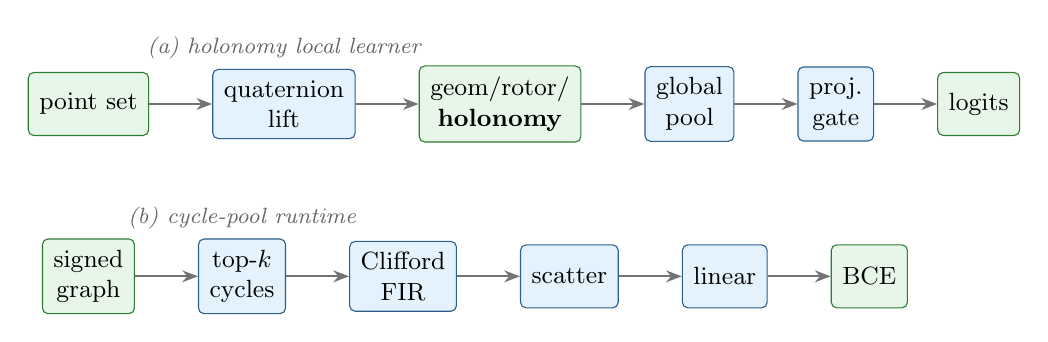
\begin{tikzpicture}[node distance=5mm and 8mm]
  \node[data] (pts) {point set};
  \node[op, right=of pts] (lift) {quaternion\\lift};
  \node[data, right=of lift] (ch) {geom/rotor/\\\textbf{holonomy}};
  \node[op, right=of ch] (pool) {global\\pool};
  \node[op, right=of pool] (gate) {proj.\\gate};
  \node[data, right=of gate] (out) {logits};
  \foreach \a/\b in {pts/lift,lift/ch,ch/pool,pool/gate,gate/out} \draw[fl] (\a)--(\b);
  \node[lbl, above=0mm of lift] {(a) holonomy local learner};
  \node[data, below=13mm of pts] (g) {signed\\graph};
  \node[op, right=of g] (cyc) {top-$k$\\cycles};
  \node[op, right=of cyc] (fir) {Clifford\\FIR};
  \node[op, right=of fir] (sc) {scatter};
  \node[op, right=of sc] (lin) {linear};
  \node[data, right=of lin] (bce) {BCE};
  \foreach \a/\b in {g/cyc,cyc/fir,fir/sc,sc/lin,lin/bce} \draw[fl] (\a)--(\b);
  \node[lbl, above=0mm of cyc] {(b) cycle-pool runtime};
\end{tikzpicture}
\caption{Two composition surfaces over the same closed-form kernels; holonomy is
the load-bearing signal in both. Closed-form local update $W\mathrel{+}=\eta\,g\,\phi\,(y-p)$.}
\end{figure}

\section{What makes it fast}\label{sec:fast}
\paragraph{No tape (structural).} A straight line of calls over \texttt{Vec<f32>}
vs a dynamic graph + tape + Python/MKL runtime. \textbf{Measured RSS $4.9$ vs
$780$ MiB ($160\times$).}

\paragraph{The \texttt{ikj}/SAXPY reorder.} The dominant matmul was a
\emph{strided-gather scalar reduction} (non-vectorisable); reordered so each input
broadcasts into a \emph{contiguous} output row, it auto-vectorises to AVX FMA and
is \textbf{bit-identical}. Measured \texttt{fused\_update} $2.9\times$, whole
forward $2.1\times$.
\begin{figure}[h]\centering
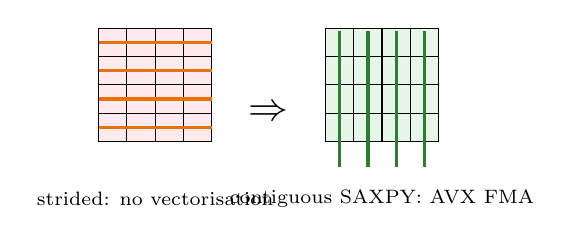
\begin{tikzpicture}[scale=0.36, every node/.style={font=\scriptsize}]
  \foreach \j in {0,...,3}\foreach \i in {0,...,3}\draw[fill=lightr] (\i,-\j) rectangle ++(1,1);
  \foreach \j in {0,...,3}\draw[nagorange,very thick] (0,-\j+0.5)--(4,-\j+0.5);
  \node at (2,-5) {strided: no vectorisation};
  \node at (6,-2) {\Large$\Rightarrow$};
  \begin{scope}[xshift=8cm]
    \foreach \j in {0,...,3}\foreach \i in {0,...,3}\draw[fill=lightg] (\i,-\j) rectangle ++(1,1);
    \foreach \i in {0,...,3}\draw[naggreen,very thick] (\i+0.5,0.9)--(\i+0.5,-3.9);
    \node at (2,-5) {contiguous SAXPY: AVX FMA};
  \end{scope}
\end{tikzpicture}
\caption{The \texttt{ikj} reorder: non-vectorisable strided reduction (left)
$\to$ contiguous broadcast-FMA (right), bit-identical.}
\end{figure}

\paragraph{Rayon MapReduce + Amdahl.} Independent rows/cycles parallelise cleanly;
MKL \emph{oversubscribes} at 32 threads ($4$--$14\times$ slower) while Nagare's
rayon scales. After the kernel fix the serial pool was the Amdahl bottleneck;
parallelising it took the parity forward $15.7\to7.6\,\mu$s/sample --- from behind
to \emph{beating} PyTorch-CPU (Fig.~\ref{fig:parity}).

\begin{figure}[h]\centering
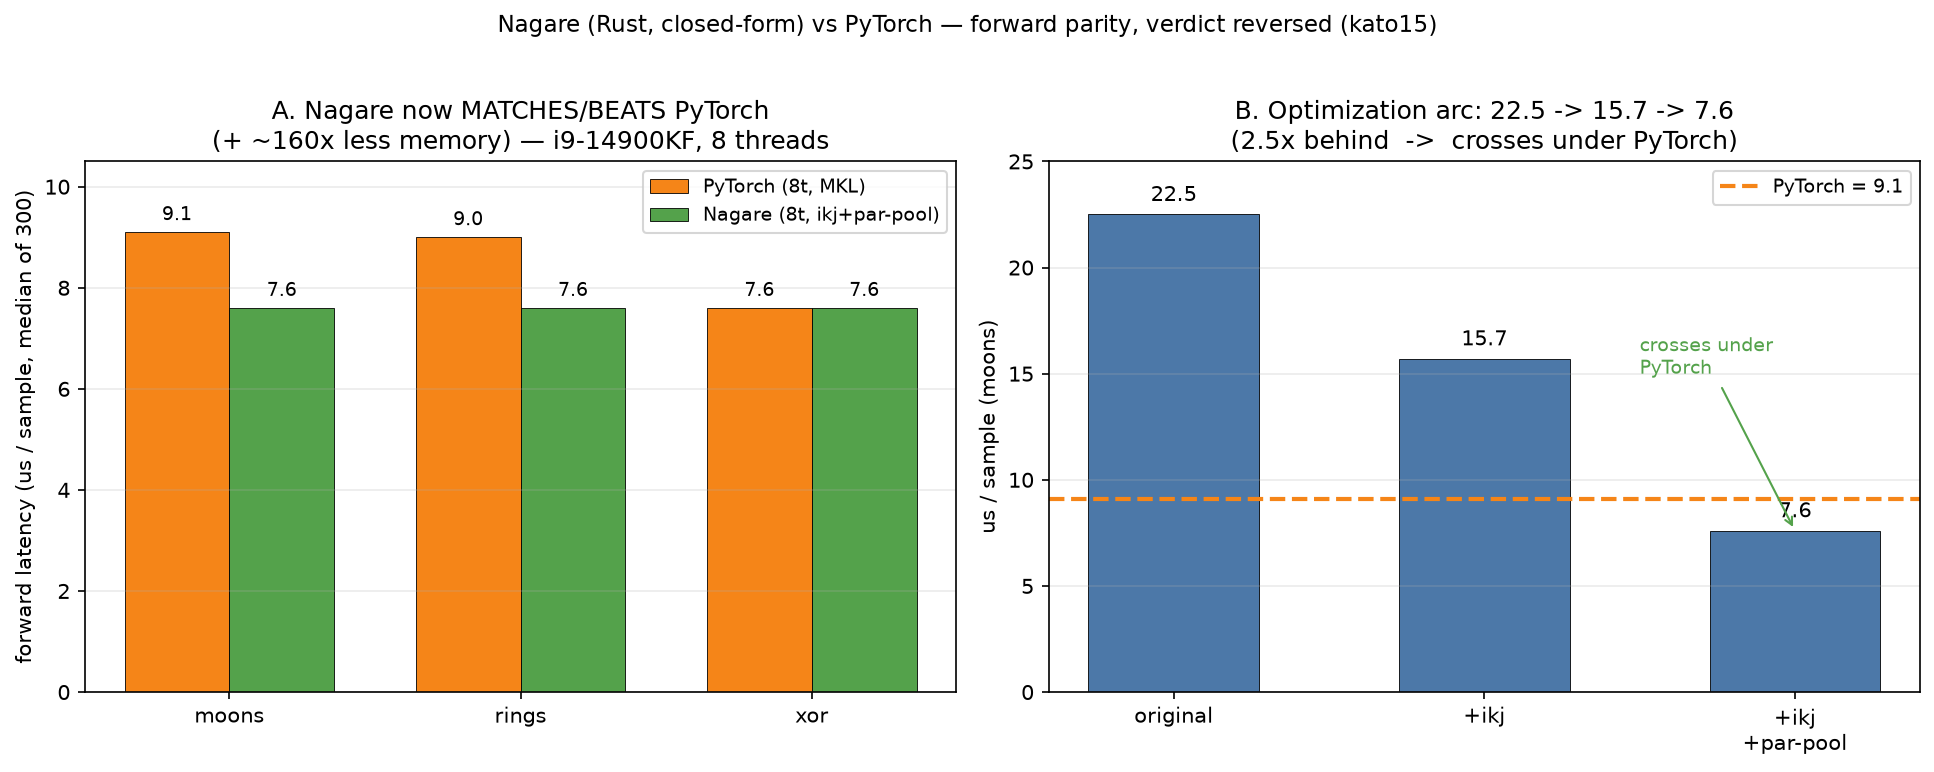
\includegraphics[width=0.86\textwidth]{2026-07-07-nagare-pytorch-parity-final-kato15.png}
\caption{\label{fig:parity}Toy-shape forward parity (kato15, 8 threads):
$22.5\to15.7\to7.6\,\mu$s/sample; Nagare crosses under PyTorch. Memory $160\times$ less.}
\end{figure}

\begin{figure}[h]\centering
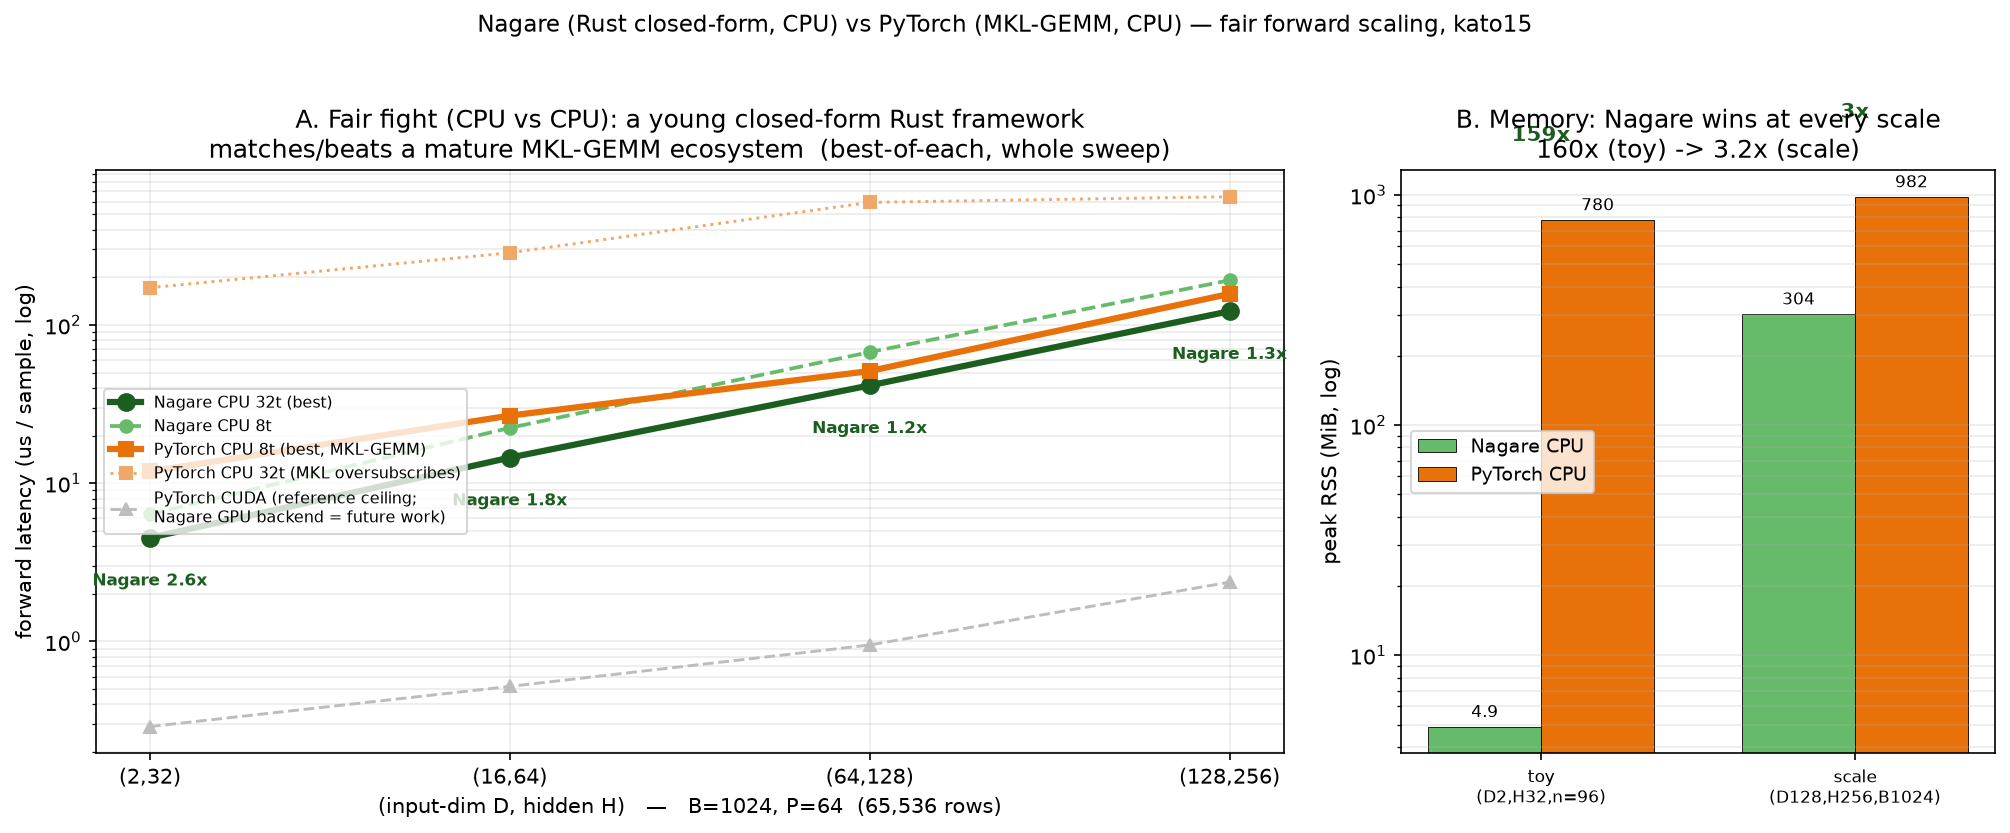
\includegraphics[width=0.92\textwidth]{2026-07-07-nagare-pytorch-scaling-kato15.png}
\caption{Fair CPU-vs-CPU dimensionality scaling: best-of-each Nagare beats
PyTorch-CPU across the whole sweep. GPU is a reference ceiling (Nagare has no GPU
backend yet), not a head-to-head. Memory edge $160\times\!\to\!3.2\times$.}
\end{figure}

\section{Holonomy = $\mathbb{Z}_2$ balance, machine-verified}\label{sec:thm}
Let $G$ be a signed graph, edge signs $s_e\in\{\pm1\}$. The \emph{holonomy} of a
cycle $C$ is $\mathrm{hol}(C)=\prod_{e\in C}s_e\in\{\pm1\}\cong\mathbb{Z}_2$.

\begin{theorem}[Cartwright--Harary; Z3-verified]
$G$ is \emph{switchable} ($\exists\sigma:V\to\{\pm1\}$ with $s_{uv}=\sigma_u\sigma_v$)
$\iff$ every cycle is positive ($\mathrm{hol}(C)=+1$).
\end{theorem}
\begin{theorem}[Gauge invariance; Z3-verified]
$\mathrm{hol}(C)$ is invariant under vertex switching; hence holonomy is a
well-defined function on the cycle space $\mathrm{GF}(2)^{m-n+1}$, not a path
artifact.
\end{theorem}
Both are proved on $K_4$ as SMT validities (unsat of the negation over \emph{all}
$2^6$ signings, not sampled); sympy confirms $\prod_{\text{cycle}}\sigma_u\sigma_v
=(\prod\sigma)^2=1$ and the cycle-space dimension over $\mathrm{GF}(2)$. Script:
\texttt{scripts/dev/holonomy\_theorems.py}.
\begin{remark}
The dimension check first failed because the incidence rank was taken over
$\mathbb{Q}$ (full rank $n$ for a non-bipartite graph) rather than $\mathrm{GF}(2)$
(rank $n-1$). The field is part of the statement.
\end{remark}

\begin{figure}[h]\centering
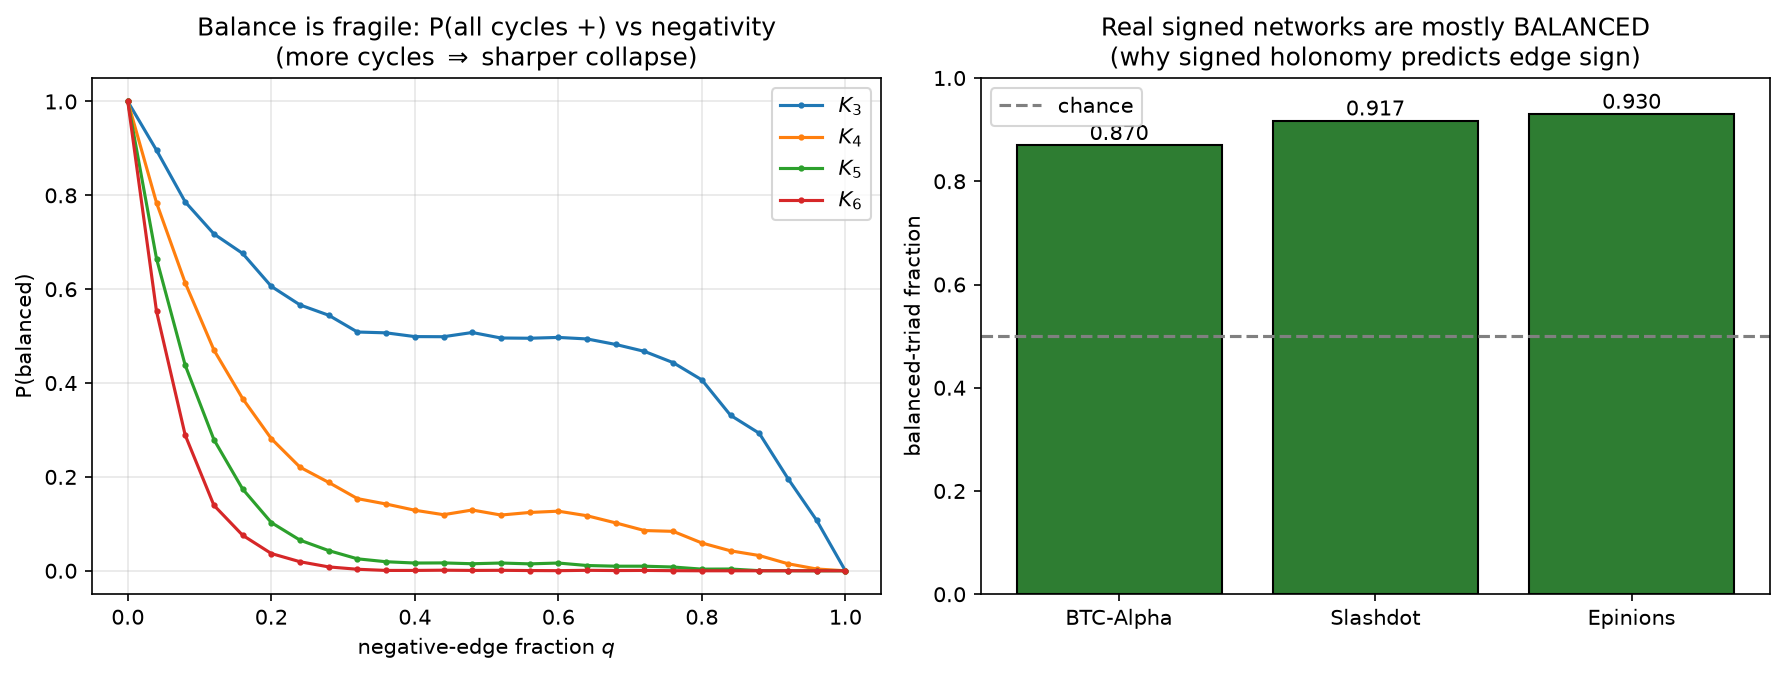
\includegraphics[width=0.92\textwidth]{2026-07-07-nagare-balance-holonomy.png}
\caption{Balance is theoretically \emph{fragile} for random signs (left;
$P(\text{balanced})$ collapses with cycle rank) yet real signed networks are
\emph{strongly} balanced (right, $0.87$--$0.93$ balanced triads). That gap is
structural balance --- and the reason signed holonomy is predictive.}
\end{figure}

\section{Signed-link prediction: the evidence chain}\label{sec:sl}
Standard protocol (SNAP Slashdot/Epinions/Bitcoin-Alpha; $80/20$ edge split;
leakage-free train-only features; Mann--Whitney AUROC; harness validated against
the literature).

\begin{table}[h]\centering\small
\begin{tabular}{lccc}
\toprule
dataset & baseline (degree) & $+$ signed holonomy & lift \\
\midrule
Bitcoin-Alpha & 0.889 & 0.901 & $+0.013$\\
Slashdot & 0.898 & 0.909 & $+0.011$\\
Epinions & 0.933 & 0.954 & $+0.021$\\
\bottomrule
\end{tabular}
\caption{Adding signed-triad holonomy ($\sum_w \mathrm{sign}(u,w)\,\mathrm{sign}(w,v)$,
i.e.\ the $\mathbb{Z}_2$ holonomy of the triad) lifts AUROC on all three ---
measured, competitive band.}
\end{table}

\noindent\textbf{But nonlinearity did \emph{not} help} at the summary-feature
level: a $64$--$64$ MLP over the same features is worse than linear
($-0.010$ to $-0.015$). So a fancier readout (Highway-KAN, spiking) \emph{over
hand-crafted holonomy summaries} is over-engineering. The open lever is a
\emph{learned} holonomy aggregation over the \emph{raw} cycle pool.

\paragraph{Depth is triad-dominated (scalar).} Multi-scale \emph{scalar}
holonomy via signed adjacency powers $A^2\!+\!A^3\!+\!A^4$ (longer signed walks)
lifts over triad-only $A^2$ only marginally, and the lift \emph{shrinks} with
density: BTC-Alpha $+0.008$, Slashdot $+0.003$, Epinions $+0.001$. On standard
signed networks the balance signal is largely triadic; deeper $\pm1$ walk
holonomy adds little once triadic closure saturates.

\paragraph{Evidence chain (state).}
(1) Theorem: signed balance $=\mathbb{Z}_2$ holonomy --- \emph{verified}.
(2) Structure: real networks are strongly balanced --- \emph{measured}.
(3) Signal: signed holonomy lifts AUROC --- \emph{measured}.
(4) Depth: \emph{scalar} deeper holonomy is triad-dominated (marginal lift) ---
\emph{measured}.
(5) \textbf{Open}: whether Nagare's \emph{rotor} (Clifford) holonomy --- the
continuous generalisation of the $\pm1$ sign product, which is a strict lower
bound of what \texttt{clifford\_fir} represents --- extracts more than scalar
walk-holonomy. That is the Nagare model's actual bet, \emph{not yet built}. The
scalar result calibrates the expectation: competitive band, depth alone marginal;
the open question is the \emph{representation} (rotor vs $\pm1$), not the order.

\section{Learning quality}
Closed-form local learner, Mann--Whitney AUROC (\texttt{examples/auroc\_eval.rs}),
$60$ parameters: clean $1.000$ on moons/spiral/xor; hard (few-shot$+$noise$+$missing)
$0.95$--$1.0$; gate-independent. Matches a backprop baseline's accuracy at
$\sim47\times$ fewer parameters. A point-order-shuffle ablation shows the
projection \emph{gate} adds no robust value --- quality comes from the pooled
features and the closed-form update, reported honestly rather than hidden.

\section{Honest bounds \& roadmap}
\begin{itemize}\itemsep1pt
  \item Matched $8$ threads, large dense matmul ($D\ge64$): tuned BLAS edges ahead
  $\sim1.2$--$1.3\times$; Nagare recovers by scaling to all cores.
  \item GPU: a reference ceiling and a defined next step (kernels are
  embarrassingly parallel), not a CPU-vs-GPU verdict.
  \item \textbf{The one rung to climb:} learned $\mathbb{Z}_2$/rotor holonomy over
  raw cycles (\texttt{clifford\_fir} over the \texttt{hymeko\_graph} cycle pool).
  Only if it lifts over linear$+$triad should a signed-KAN readout, tree
  compression / entropy routing, or a Steiner/AG$(2,3)$ group generalisation be
  tested --- each gated by a discriminating ablation and a novelty search.
\end{itemize}

\section{Reproducibility}
$45$ tests green (Windows + Linux/kato15); clippy/fmt clean; bit-identical
optimisations proven by a frozen seed-$53$ fixture, finite-difference tests, and
the order-shuffle mechanism test. Self-contained (vendored \texttt{hymeko\_clifford}
$+$ \texttt{hymeko\_graph}). Harnesses: \texttt{examples/\{forward\_profile,
scaling\_bench, auroc\_eval, toy\_compare\}.rs}; \texttt{scripts/dev/\{signed\_link\_baseline,
signed\_link\_holonomy, signed\_link\_nonlinear, holonomy\_theorems, scaling\_bench\_torch\}.py}.

\end{document}
